\documentclass[titlepage, a4paper, 12pt]{article}
\usepackage[swedish]{babel}
\usepackage[utf8]{inputenc}
\usepackage{verbatim}
\usepackage{fancyhdr}
\usepackage{graphicx}
\usepackage{parskip}

% SourceCode
\usepackage{listings}
\usepackage{color}

% Include pdf with multiple pages ex \includepdf[pages=-, nup=2x2]{filename.pdf}
\usepackage[final]{pdfpages}
% Place figures where they should be
\usepackage{float}

% SourceCode
\definecolor{keywordcolor}{rgb}{0.5,0,0.75}
\lstset{
  inputencoding=utf8,
  language=Java,
  extendedchars=true,
  basicstyle=\scriptsize\ttfamily,
  stringstyle=\color{blue},
  commentstyle=\color{red},
  numbers=left,
  firstnumber=auto,
  numberblanklines=true,
  stepnumber=1,
  showstringspaces=false,
  keywordstyle=\color{keywordcolor}
  % identifierstyle=\color{identifiercolor}
}

% Float for text
\floatstyle{ruled}
\newfloat{kod}{H}{lop}
\floatname{kod}{Kodsnutt}

% vars
\def\title{Boids}
\def\preTitle{Laboration 2}
\def\kurs{Emergenta system, VT-09}

\def\namn{Andreas Jakobsson}
\def\mail{dit06ajs@cs.umu.se}
\def\namnTva{Anton Johansson}
\def\mailTva{dit06ajn@cs.umu.se}

\def\pathtocode{$\sim$dit06ajn/edu/emergenta-system/lab2/src}

\def\handledareEtt{Jonny Pettersson, jonny@cs.umu.se}
\def\handledareTva{Anders Broberg, bopspe@cs.umu.se}

\def\inst{datavetenskap}
\def\dokumentTyp{Laborationsrapport}

\begin{document}
\begin{titlepage}
  \thispagestyle{empty}
  \begin{small}
    \begin{tabular}{@{}p{\textwidth}@{}}
      UMEÅ UNIVERSITET \hfill \today \\
      Institutionen för \inst \\
      \dokumentTyp \\
    \end{tabular}
  \end{small}
  \vspace{10mm}
  \begin{center}
    \LARGE{\preTitle} \\
    \huge{\textbf{\kurs}} \\
    \vspace{10mm}
    \LARGE{\title} \\
    \vspace{15mm}
    \begin{large}
      \namn, \mail \\
      \namnTva, \mailTva\\
      \texttt{\pathtocode}
    \end{large}
    \vfill
    \large{\textbf{Handledare}}\\
    \mbox{\large{\handledareEtt}}
    \mbox{\large{\handledareTva}}
  \end{center}
\end{titlepage}

\newpage
\mbox{}
\vspace{70mm}
\begin{center}
% Dedication goes here
\end{center}
\thispagestyle{empty}
\newpage

\pagestyle{fancy}
\rhead{\today}
\lhead{\footnotesize{\namn, \mail\\\namnTva, \mailTva}}
\chead{}
\lfoot{}
\cfoot{}
\rfoot{}

\cleardoublepage
\newpage
\tableofcontents
\cleardoublepage

% \fancyfoot[LE,RO]{\thepage}
\cfoot{\thepage}
\pagenumbering{arabic}

\section{Problemspecifikation}\label{sec:problemspecifikation}
Laborationen gick ut på att göra ändringar i en befintlig
NetLogo\footnote{http://ccl.northwestern.edu/netlogo/} modell som
imiterar flockbete. Modellen utvecklades av Craig Reynolds på 80-talet
och varje individ, så kallad \textit{boid}, följer tre enkla regler:

\begin{itemize}
\item Undvik kollision med grannar.
\item Håll samma hastighet och riktning som dina grannar.
\item Försök ha en  position så nära centrum av flocken som möjligt.
\end{itemize}

Denna modell ska utökas så att flockarna ska kunna undvika hinder i
dess väg, och att de istället för att röra sig slumpvis omkring i
miljön ska kunna röra sig mot ett gemensamt mål som bestäms av
muspekarens position.

\subsection{Frågor som ska behandlas}
I problemspecifikationen finns följande frågor som denna rapport ska
behandla.

\textbf{Hinder:}
\begin{itemize}
\item Vad krävs för att en flock ska kunna splittras upp när de
  undviker ett hinder och gå ihop till en samlad flock när hindret är
  passerat?
\item Vilken metod valde ni och varför?
\item Hur skulle er metod fungera med andra hinder än punktformade?
\item Finns det någon gräns för hur stora hindren kan vara?
\end{itemize}

\textbf{Mål:}
\begin{itemize}
\item Modellen ska utvidgas till att inkludera ett gemensamt mål,
  alltså en punkt eller yta i världen som alla boids strävar efter att
  nå.
\item Minimikravet är att man ska kunna ställa in målet genom att med
  muspekaren välja en punkt i världen
\item Hur bibehålls flockbeteendet när ett mål finns?
\item Hur stor vikt bör man lägga på mål, hinder och flockbeteende för
  att få ett beteende som ser naturligt ut?
\item Vilken sorts beteende anser ni är naturligt eller önskvärt? 
\end{itemize}

Laborationsspecifikation finns i original på sidan:\\
\verb!http://www.cs.umu.se/kurser/5DV017/VT09/lab/lab2.html!


\section{Användarhandledning}
Källkoden till implementationen Flocking.nlogo som diskuteras i denna
rapport finns att hitta på:

\verb!~dit06ajn/edu/emergenta-system/lab2/src!

Öppna filen i NetLogo för att köra den.

\subsection{Förklaring av användargränssnittet}
Nedan följer en förklaring av de knappar och reglage som förekommer i
användargränssnittet:

\begin{itemize}
\item \textbf{population} - antalet individer i världen.
\item \textbf{nr-of-obstacles} - antalet hinder i världen.
\item \textbf{setup} - denna knapp initierar parametrarna till världen.
\item \textbf{go} - denna knapp sätter igång animeringen i
  världen. Setup måste köras en gång innan denna knapp får användas.
\item \textbf{vision-radius} - antalet rutor en individ kan se.
\item \textbf{vision-angle} - vinkeln för en individs synfält angett i
  grader.
\item \textbf{minimum-seperation} - det minsta avståndet en individ
  vill ha till sina grannar angett i rutor.
\item \textbf{max-align-turn} - den maximala vinkeln en individ kan
  svänga för att komma i samma färdriktning som sina grannar.
\item \textbf{max-cohere-turn} - den maximala vinkeln en individ kan
  svänga för att komma närmare mittpunkten av sina grannar.
\item \textbf{max-seperate-turn} - den maximala vinkeln en individ kan
  svänga för att komma längre bort från sin närmsta granne.
\item \textbf{max-avoidance-turn} - den maximala vinkeln en individ
  kan svänga för att undvika ett hinder.
\item \textbf{moving-obstacles?} - om denna är på förflyttar sig
  hindren i slumpmässig riktning.
\item \textbf{follow-mouse?} - om denna är på försöker individerna att
  följa efter muspekaren om den befinner sig inom världens gränser.
\item \textbf{max-goal-turn} - den maximala vinkel en individ får
  använda sig av för att svänga mot muspekaren.
\end{itemize}

Avstånd är mätt i antal rutor i världen, vinklar är mätt i grader.

\section{Algoritmbeskrivning}
Nedan avsnitt beskriver de algoritmer som implementerats för att
införa hinderavvikelse och målsökande i modellen.

\subsection{Hinder}\label{algo:hinder}
För att flockarna ska kunna undvika hinder har det införts nya agenter
härefter refererade som \textit{hinder}. Varje individ fått en ny
procedur \textit{obstacle-avoidance} som utförs före att de har utfört
sitt flock-beteende.

Metoden \textit{steer-to-avoid} implementerades där hinderundvikande
löses genom att varje individ letar efter det närmaste hinder som
befinner sig i en kon i deras färdriktning, se figur
\ref{fig:collision}. Konens storlek bestäms av variablerna
\textit{vision-radius} och \textit{vision-angle}. Om ett hinder
upptäckts i konen svänger individen bort från denna med en vinkel som
beräknas enligt \textit{max-avoidance-turn} delat med avståndet till
hindret. Detta innebär att enheten vid tidig upptäckt av hinder
svänger minimalt, när enheten närmar sig hindret ökar vinkeln den
försöker svänga bort med. Den initiala vinkeln, se \textit{v} i figur
\ref{fig:collision}, individen har mot målet i förhållande till sin
färdriktning används för att bestämma vilket håll om hindret individen
ska välja för att förhindra kollision. Om \textit{v} är negativ
svänger individen åt vänster, annars åt höger.

\begin{figure}[H]
  \begin{center}
    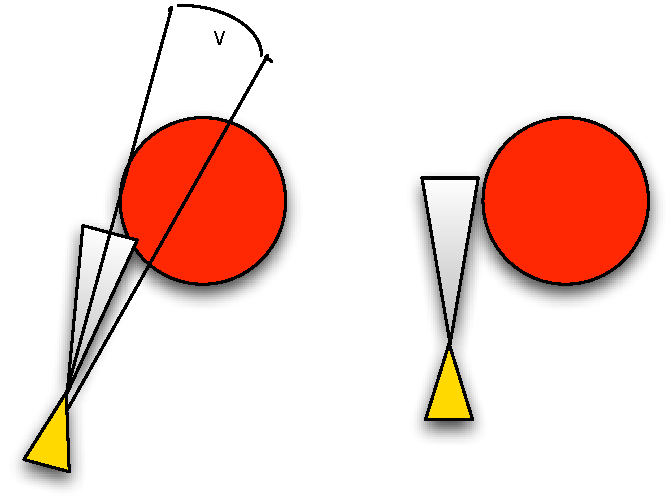
\includegraphics[width=110mm]{images/collision.pdf}
    \caption{Kollisionshantering}
    \label{fig:collision}
  \end{center}
\end{figure}

\subsection{Mål}
För att få flockarna att söka sig mot ett gemensamt mål
implementerades proceduren \textit{find-goal} som räknar ut vinkeln
mot målet, representerat av mus\-pekarens position. Individerna svänger
mot målet i varje tidssteg med maximalt tillåten vinkel,
\textit{max-goal-turn}.

\section{Strategi för testning}
Under laborationens gång används trial-and-error för att testa ifall
koden genererar önskade beteenden. För att få svar på frågorna görs
försök till att upprepa samma situation flera gånger med olika
parameterinställningar för att subjektivt bedömma hur parametrarna
påverkar beteenden. För återskapa beteenden som diskuteras i rapporten
ombeds testkörningar med programmet där parametrar ändras på det sätt
som beskrivs i avsnitt \ref{sec:reflektioner}.

Några skärmdumpar presenteras som diskussionsunderlag till beteenden.

\section{Reflektioner}\label{sec:reflektioner}
% Rapportens huvudsyfte är att redovisa era reflektioner kring det som
% laborationen behandlar, dvs reflektionsdelen är viktig.  Diskutera
% de frågor som nämns ovan och försöka att sätta in laborationen i ett
% större sammanhang. Vilka applikationsområden kan du se för den här
% typen av algoritmer?  Kan modellen utöka för att göras mer
% intressant?

% I er rapport ska följande punkter tas med:

%     * Ett fullständigt försättsblad
%     * Sökvägen till er NetLogo-kod (kan skrivas på försättsbladet)
%     * Reflektion kring er lösning och eventuella begränsningar
%     * Reflektion kring de frågor som ställs ovan samt saker som
%       du själv finner relevant. Ta gärna hjälp av skärmdumpar.
%     * Utskriven dokumenterad källkod
Nedan avsnitt beskriver reflektioner som gjorts med avseende på
frågorna från problemspecifikationen.

\subsection{Hinder}
% Vad krävs för att en flock ska kunna splittras 
%     upp när de undviker ett hinder och gå ihop
%     till en samlad flock när hindret är passerat?
För att en flock ska splittras vid ett hinder och sedan samlas ihop
igen på andra sidan hindret krävs att individerna har tillräckligt
stor sikt för att kunna upptäcka individer som tvingades välja en
annan väg runt hindret. Anledningen till att individerna återförenas i
en flock efter de har stött på ett hinder är deras
\textit{coherence}-beteende gör att de strävar mot en gemensam
mittpunkt för flocken. Se figur \ref{fig:flock} för en sekvens där en
flock möter ett hinder, inställningar för simulering finns i bilaga
\ref{app:flock}.

\begin{figure}[H]
  \begin{center}
    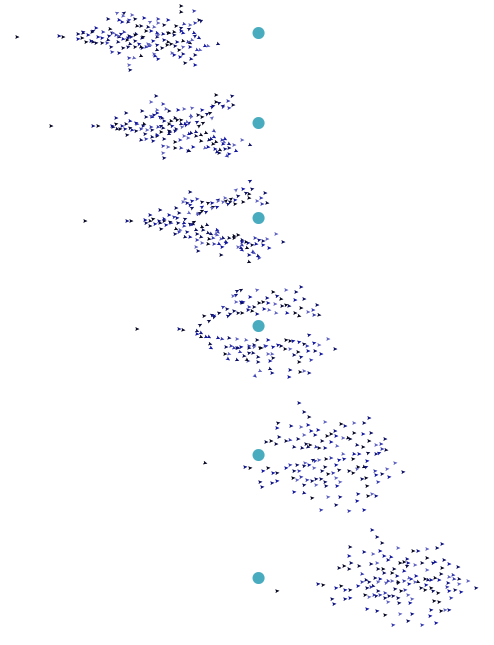
\includegraphics[width=110mm]{images/flock.png}
    \caption{Kollisionshantering för flock}
    \label{fig:flock}
  \end{center}
\end{figure}

Många parametrar spelar in vid återförening av flocken efter
hinder. Om vinkeln mellan de två flockarna är stor samtidigt som
individernas \textit{cohere-turn}-parameter är låg kan flockarna
återförening utebli även fast de initialt såg varandra när hindret
forcerats. Detta eftersom de inte hinner svänga mot varandra innan
deras synfällt upphör att sammanfalla.

% Vilken metod valde ni och varför?
Vi valde att implementera ett \textit{steer-to-avoid}-beteende, se
avsnitt \ref{algo:hinder}, till skillnad från
\textit{force-field}-beteende som skulle innebära att ett hinder
stöter bort enheten oberoende av enhetens riktning. Beteendet
\textit{steer-to-avoid} innebär att en individ kan röra sig parallellt
med ett hinder utan att påverkas av det. Detta är viktigt för
återförenande av flockar efter hinder. Notera dock att sätts vinkeln
\textit{vision-angle} till ett stort värde nära 360 grader kommer
denna metod att likna \textit{force-field}-metoden i och med att
individen påverkas av hinder som inte enbart ligger framför dess
färdriktning.

I nuläget är hindret implementerat som en cirkel med en diameter
motsvarande storleken. När vinkel mellan en individ och ett hinder
beräknas betraktas hindrets mittpunkt och hänsyn kommer inte tas till
hindrets storlek. Däremot beräknas avståndet till hindret som
mittpunkt på hindret - radien för att få ett hinder med en
cirkulär yta.

% Hur skulle er metod fungera med andra hinder än punktformade?
% Finns det någon gräns för hur stora hindren kan vara?
Eftersom vår modell använder sig av den inbyggda metoden
\textit{in-cone} för att upptäcka hinder i en individs synfält används
hindrens mittpunkt vid detektion. Detta innebär en begränsning som gör
att storleken på hindrena inte får överstiga en enhets parametervärde
på \textit{vision-radius}. Om så är fallet kommer individen att krocka
redan innan den har upptäckt hindret den krockar med.

\subsection{Mål}
% Modellen ska utvidgas till att inkludera ett gemensamt mål,
%           alltså en punkt eller yta i världen som alla boids
%           strävar efter att nå.
%           Minimikravet är att man ska kunna ställa in målet genom att
%             med muspekaren välja en punkt i världen
% Hur bibehålls flockbeteendet när ett mål finns?
När modellen utökades för att få individerna att söka sig mot ett
gemensamt mål blev det svårare att avskilja vad som är flockbeteende
och vad som är målsökarbeteende. Eftersom alla strävar mot samma mål
får närliggande individer samma riktning. Om man minskar på parametern
som anger en individs maxsväng mot mål, \textit{max-goal-turn},
upplevs flockbeteendet starkare eftersom individernas svängar för
flockbeteende får högre dominans än individernas målsökande svängar.

% Hur stor vikt bör man lägga på mål, hinder och flockbeteende
% för att få ett beteende som ser naturligt ut?
I våra testkörningar har vi noterat att balansen mellan mål- och
flockbeteende är avgörande för hur naturlikt simuleringen verkar. Med
naturlikt menar vi flockbeteende som kan ses bland fåglar och
fiskar. Vi anser då att det bör läggas störst vikt vid att undvika
hinder, det vill säga att i simuleringen tillåta individerna en stor
vinkel på \textit{max-avoidance-turn}. Därefter bör det läggas större
vikt på flockbeteende än på målsökarbeteende. Vi gör jämförelsen med
flyttfåglar där målsökandet är något som kontinuerligt sker över en
större tidsperiod än flockbeteendet, som är en mer aktiv process.

% DONE Vilken sorts beteende anser ni är naturligt eller önskvärt? 

\newpage
\appendix
\pagenumbering{roman}
\section{Källkod}\label{sec:kallkod}
% Källkoden ska finnas tillgänglig i er hemkatalog
% ~/edu/apjava/lab1/. Bifoga även utskriven källkod.
Härefter följer utskrifter från källkoden och andra filer som hör till
denna laboration

\subsection{Paremeterinställningar för figur \ref{fig:flock}}\label{app:flock}
\begin{itemize}
\item \textbf{population} - 140
\item \textbf{nr-of-obstacles} - 1
\item \textbf{vision-radius} - 20
\item \textbf{vision-angle} - 50
\item \textbf{minimum-seperation} - 1
\item \textbf{max-align-turn} - 2.75
\item \textbf{max-cohere-turn} - 2.75
\item \textbf{max-seperate-turn} - 1
\item \textbf{max-avoidance-turn} - 90
\item \textbf{moving-obstacles?} - off
\item \textbf{follow-mouse?} - off
\item \textbf{max-goal-turn} - 2.5
\end{itemize}

\subsection{Flocking.nlogo}\label{app:Flocking.nlogo}
\begin{footnotesize}
  \verbatiminput{../src/Flocking.nlogo}
\end{footnotesize}

\end{document}
